%%%%%%%%%%%%%%%%%%%%%%%%%%%%%%%%%%%%%%%%%
% Short Sectioned Assignment
% LaTeX Template
% Version 1.0 (5/5/12)
%
% This template has been downloaded from:
% http://www.LaTeXTemplates.com
%
% Original author:
% Frits Wenneker (http://www.howtotex.com)
%
% License:
% CC BY-NC-SA 3.0 (http://creativecommons.org/licenses/by-nc-sa/3.0/)
%
%%%%%%%%%%%%%%%%%%%%%%%%%%%%%%%%%%%%%%%%%

%----------------------------------------------------------------------------------------
%	PACKAGES AND OTHER DOCUMENT CONFIGURATIONS
%----------------------------------------------------------------------------------------

\documentclass[paper=a4, fontsize=11pt]{scrartcl} % A4 paper and 11pt font size

\usepackage[T1]{fontenc} % Use 8-bit encoding that has 256 glyphs
\usepackage{fourier} % Use the Adobe Utopia font for the document - comment this line to return to the LaTeX default
\usepackage[english]{babel} % English language/hyphenation
\usepackage{amsmath,amsfonts,amsthm} % Math packages
\usepackage{lipsum} % Used for inserting dummy 'Lorem ipsum' text into the template
\usepackage{placeins}
\usepackage{sectsty} % Allows customizing section commands
\usepackage{amsmath} % Mathematic Library
\allsectionsfont{\textbf\normalfont\scshape} % Make all sections centered, the default font and small caps

\usepackage{fancyhdr} % Custom headers and footers
\usepackage{listings}
\usepackage{xcolor}
\usepackage{caption}
\usepackage{graphicx}
\usepackage{multirow}

\definecolor{dkgreen}{rgb}{0,0.6,0}
\definecolor{gray}{rgb}{0.5,0.5,0.5}
\definecolor{mauve}{rgb}{0.58,0,0.82}

\lstdefinestyle{mycode} {
  frame=tb,
  language=C,
  aboveskip=3mm,
  belowskip=3mm,
  showstringspaces=false,
  columns=flexible,
  basicstyle={\small\ttfamily},
  numbers=left,
  numberstyle=\tiny\color{gray},
  keywordstyle=\color{blue},
  commentstyle=\color{dkgreen},
  stringstyle=\color{mauve},
  frame=single,
  breaklines=true,
  breakatwhitespace=true,
  tabsize=1,
}

\pagestyle{fancyplain} % Makes all pages in the document conform to the custom headers and footers
\fancyhead{} % No page header - if you want one, create it in the same way as the footers below
\fancyfoot[L]{} % Empty left footer
\fancyfoot[C]{} % Empty center footer
\fancyfoot[R]{\thepage} % Page numbering for right footer
\renewcommand{\headrulewidth}{0pt} % Remove header underlines
\renewcommand{\footrulewidth}{0pt} % Remove footer underlines
\setlength{\headheight}{13.6pt} % Customize the height of the header

\numberwithin{equation}{section} % Number equations within sections (i.e. 1.1, 1.2, 2.1, 2.2 instead of 1, 2, 3, 4)
\numberwithin{figure}{section} % Number figures within sections (i.e. 1.1, 1.2, 2.1, 2.2 instead of 1, 2, 3, 4)
%\numberwithin{table}{section} % Number tables within sections (i.e. 1.1, 1.2, 2.1, 2.2 instead of 1, 2, 3, 4)

\setlength\parindent{0pt} % Removes all indentation from paragraphs - comment this line for an assignment with lots of text

%----------------------------------------------------------------------------------------
%	TITLE SECTION
%----------------------------------------------------------------------------------------

\newcommand{\horrule}[1]{\rule{\linewidth}{#1}} % Create horizontal rule command with 1 argument of height

\title{	
\normalfont \normalsize 
\textsc{University of Crete, Computer Science Department} \\ [25pt] % Your university, school and/or department name(s)
\horrule{0.5pt} \\[0.4cm] % Thin top horizontal rule
\huge CS-486 -- Principles of Distributed Systems \\
1st Set of Exercises: Theory Part % The assignment title
\horrule{2pt} \\[0.5cm] % Thick bottom horizontal rule
}

\author{Iacovos Kolokasis \\(kolokasis@csd.uoc.gr) \\AM:1039} % Your name

\date{\normalsize\today} % Today's date or a custom date

\begin{document}

\maketitle % Print the title
\section*{Exercise A}

\paragraph{1a.}
This algorithm presents the fair synchronization algorithm which uses
some key ideas from Black-White Bakery algorithm. $P_i$ to get in its
entry section of the critical section (CS) reads the value of the
group and determines which of the two groups (0 or 1) it should
belong. When the $P_i$ chooses a group, it waits until its group has
priority over the other group and then it enters to the CS. 
The order of which processes can enter to the CS is defined as
follows:%
(1) if two processes belong to two different groups, the process whose
group as recorded in its state is different from the value of group is
enabled and can enter to the CS and the other process has to wait, and
%
(2) if all the active processes belong to the same group then they can
all enter to the CS.
When a process exits from the CS set the group bit to a value which is
different from the value of its state. Thus, exit process ($P_i$)
gives priority to waiting processes which belong to the same group
that $P_i$ process belongs to.

\bigskip
Our algorithm needs to ensure for correct synchronization that two
waiting process $P_i$ and $P_j$, if $state[i] \neq group$ and
$state[j] = group$ then $P_i$ must enter the CS and completes its exit
section before $P_j$ enters its CS. 

\bigskip
A process $P_i$ is enabled to
enter its CS only when one of the following conditions are met: %
(1) the value of $state_i \neq group$, in such case, $P_i$ will break
out the for loop in line 4; or %
(2) for all processes $state[j] \neq 1 - state[i]$ where no process
belong to a different group than the group that $P_i$ belongs to. In
that case, $P_i$ will execute the loop $n$ times and will exit.
If none of these two conditions are true, $P_i$ will have to wait in
line 7, until the value of the group changes or the process $P_j$ of
that belongs to the other group changes its value.
The process $P_j$ can become enabled until the value of the group
change or all the processes of the group of $P_i$ complete their CS.

\paragraph{1b.}
Assume a beginning process $P_i$ overtakes a waiting process $P_j$ in
entering its critical section.  This can happen only if both $P_i$ and
$P_j$ belong to the same group at the time when $P_i$ has completed
executing line 2.  During the exit section of the CS $P_i$ will set
the value of the group to $1 - state[i]$.  Thereafter, by the
value of the group will not change until $P_j$ completes its exit
section.  If $P_i$ tries to enter to the CS again while $P_j$ has not
completed its exit section yet, then after passing through line 1
$P_i$ will belong to a different group than $P_j$ and the value of the
group bit will be the same as the value of $state[i]$. Thus $P_i$ will
not become enabled again until $P_j$ completes its exit section and
changes the value of its state $P_j$. Thus, the algorithm satisfies
fairness.

\paragraph{1c.}
If we omit line 1 and 5 will result in an incorrect algorithm. Line 1
and 5 ensures that a process has started executing its doorway code.
If we remove these two lines then a none beginning process $P_i$ may
enter in CS ahead of another waiting process $P_j$ twice: the first
time if $P_i$ is running on the other group and the second time if
$P_i$ pass $P_q$ which is waiting on the same group and enters in CS
first.

\paragraph{1d.}
Line 4 is used to ensure priority between the groups.

\paragraph{2.}
Solution for the first part of the exercise:

\begin{lstlisting}[style=mycode]

shared variables
int array[c], next_ticket, now_serving, desks, current_ticket, counter;

void hospital()
{
	int my_ticket	
	my_ticket = fetch_and_incr(next_ticket)

	while (now_serving != my_ticket);

	while (counter == 0);

	fetch_and_decr(counter)

	while (desks == 0);

	fetch_and_decr(desks)
	
	// Fill documents 

	fetch_and_incr(desks)

	int i = 0;

	while (true)
	{
		if (array[i].lock != 1)
		{
			lock(array[i])
			break;
		}
		i++;

		i (i >= c)
		{
			i = 0;
		}
	}

// CS

	unlock(array[i])

	fetch_and_incr(counter)
}

\end{lstlisting}

\paragraph{2.}
Solution for the second part of the exercise (graduate):

\begin{lstlisting}[style=mycode]
entry_section()
{

shared variables
int array[c], next_ticket, now_serving, desks, current_ticket, counter;

void hospital()
{
	int my_ticket	
	my_ticket = fetch_and_incr(next_ticket)

	while (now_serving != my_ticket);

	while (counter == 0);

	fetch_and_decr(counter)

	while (desks == 0);

	fetch_and_decr(desks)
	
	// Fill documents 

	fetch_and_incr(desks)

	int i = 0;

	while (true)
	{
		if (array[i].lock != 1)
		{
			lock(array[i])
			break;
		}
		i++;

		i (i >= c)
		{
			i = 0;
		}
	}

	while (worker[my_ticket % w].lock == 1);
	
	fetch_and_incr(worker[my_ticket % w].lock);

	fetch_and_incr(samples)

	unlock(array[i])

	fetch_and_incr(counter)
}

\end{lstlisting}

\section*{Exercise B}
\paragraph{1.}
If we delete the line \textbf{pred.next = curr} then we will have the
following scenarios where the thread is going through nodes that have
been removed and thus, pred can point to a node already removed. 

\textbf{Example:}
If we have a list with 3 elements: 10, 40, and 50. The tread A try to
delete the node in 40 while the thread B try to insert the node 45
between node 40 and 50. While the thread B tries to insert the new
node does not see the new \textbf{pred.next = curr} as a result to
connect the new node with the already deleted node 40.

\paragraph{2}
In the case of the Lazy algorithm, canceling the flag marked
invalidates the validate() and contains() method that depend on this
mark.

\paragraph{3}
No, we cannot modify the insert() method of the fine-grained
synchronization list so that it locks only on node because we need to
lock the previous node and the current node each time. During the
insertion path the previous node will point to the new node and the
new node will point to the current node. In the possibility of keeping
only one lock in the current node then two threads might try to add a
new node to the previous node which that is not correct. 

\section*{Exercise C}

\begin{lstlisting}[style=mycode]

// Node structure
struct Node {
	int _key;               // Node key
	struct Node *left;      // Left child
	struct Node *right;     // Right child
	struct Node *l_thread;  // Left threaded
	struct Node *r_thread;  // Right threaded
};

// Insert a Node in Binary Threaded Tree 
struct Node *BSTInsert(struct Node *root, int ikey) 
{ 
    Node *ptr; 
    Node *par = NULL;		// Parent node
	Node *child = NULL;	// Child node

    // Searching for a Node with given value 
	lock(root);
	ptr = root

    while (ptr != NULL) 
    { 
        // If key already exists, return 
        if (ikey == (ptr->info)) 
        { 
			unlock(root);
            return ptr; 
        } 
  
        par = ptr;	// Update parent pointer 
  
        // Moving on left subtree. 
        if (ikey < ptr->info) 
        { 
            if (ptr->l_thread == false) 
				child = ptr->left
				lock(child)
                ptr = child
            else
                break; 
        } 
  
        // Moving on right subtree. 
        else
        { 
            if (ptr->r_thread == false) 
				child = ptr->right;
				lock(child);
                ptr = child;
            else
                break; 
        } 

		unlock(par);
    } 
  
    // Create a new node 
    Node *tmp = new Node; 
    tmp->info = ikey; 
    tmp->l_thread = true; 
    tmp->r_thread = true; 
  
    if (par == NULL) 
    { 
        root = tmp; 
        tmp->left = NULL; 
        tmp->right = NULL; 
		unlock (par);
		return root;
    } 
    else if (ikey < (par->info)) 
    { 
        tmp->left = par->left; 
        tmp->right = par; 
        par->l_thread = false; 
        par->left = tmp; 
    } 
    else
    { 
        tmp->left = par; 
        tmp->right = par->right; 
        par->r_thread = false; 
        par->right = tmp; 
    } 

	unlock(par)
	unlock(root)
  
    return root; 
} 

// Insert a Node in Binary Threaded Tree 
struct Node *BSTSearch(struct Node *root, int ikey) 
{ 
    Node *ptr; 
    Node *par; 
    Node *child; 

    // Searching for a Node with given value 
	lock(root);
	ptr = root

    while (ptr != NULL) 
    { 
        // If key already exists, return 
        if (ikey == (ptr->info)) 
        { 
			unlock(ptr);
            return ptr; 
        } 

		par = ptr
  
        // Moving on left subtree. 
        if (ikey < ptr->info) 
        { 
            if (ptr->l_thread == false) 
				child = ptr->left
				lock(child)
                ptr = child
            else
                break; 
        } 
  
        // Moving on right subtree. 
        else
        { 
            if (ptr->r_thread == false) 
				child = ptr->right;
				lock(child);
                ptr = child;
            else
                break; 
        } 

		unlock(par);
    } 
} 

// Insert a Node in Binary Threaded Tree 
struct Node *BSTSearch(struct Node *root, int ikey) 
{ 
    Node *ptr; 
    Node *par; 
    Node *child; 

    // Searching for a Node with given value 
	lock(root);
	ptr = root

    while (ptr != NULL) 
    { 
        // If key already exists, return 
        if (ikey == (ptr->info)) 
        { 
			unlock(ptr);
            return ptr; 
        } 

		par = ptr
  
        // Moving on left subtree. 
        if (ikey < ptr->info) 
        { 
            if (ptr->l_thread == false) 
				child = ptr->left
				lock(child)
                ptr = child
            else
                break; 
        } 
  
        // Moving on right subtree. 
        else
        { 
            if (ptr->r_thread == false) 
				child = ptr->right;
				lock(child);
                ptr = child;
            else
                break; 
        } 

		unlock(par);
    } 
} 

// Delete a Node in Binary Threaded Tree 
struct Node *BSTDelete(struct Node *root, int ikey) 
{ 
    Node *ptr; // Current pointer
    Node *par; // Parent pointer
    Node *child; // Child pointer
	int found = 0;	// Key is found 

    // Searching for a Node with given value 
	lock(root);
	ptr = root

	// Search the key
    while (ptr != NULL) 
    { 
		if (dkey == ptr->info)
		{
			found = 1
			break;
		}

		par = ptr

		if (dkey < ptr->info)
		{
			if (ptr->lthread == false)
			{
				child = ptr->left;
				lock(child);
			}
			else
				break;
		}
		else {
			if (ptr->rthread == false)
			{
				child = ptr->right;
				lock(child);
			}
			else
				break;
		}

		unlock(par);
	} 

	if (found == 0)
		printf("The key does not found");

	else if (ptr->lthread == false && ptr->rthread == false)
	{
		struct Node* par_succ = ptr;
		struct Node* succ = ptr->right;

		lock(succ);

		while (succ->left != NULL)
		{
			parsucc = succ;
			succ = succ->left;
			lock(suck)
		}

		ptr->key = succ->key
	}

\end{lstlisting}

\paragraph{2.}
We implement a fine-grain locking for the lock-based implementation of
the concurrent threaded binary search tree. In our implementation we
lock the parent node, the current node and the child node of each
visit node.

\paragraph{3.}
Let us have the scenario that I have a null tree, then add a new key
and then I delete this key. As a result we will have a null tree
again.
Liniarization points in Insertion: line 69 or line 88 where the new
element is already inserted in the tree.
Liniarization points in Deletion: line xx or line xx.


\paragraph{4.}
The algorithm is correct because for each node that we traverse we
lock the parent node and the child node. By keeping these three nodes
locked during insertion and deletion operation we ensure that we are
going to perform correctly each one operation.

\paragraph{5.}


\paragraph{6.}

\section*{Exercise 4A}

\begin{table}[h]
\begin{tabular}{cc}
\hline
\multicolumn{1}{|l|}{\textbf{Event A}} & \multicolumn{1}{l|}{\textbf{Event B}} \\ \hline
\multicolumn{1}{|c|}{$\varphi{16}$}                 & \multicolumn{1}{c|}{$\varphi{3}$}                 \\ \hline
\multicolumn{1}{|c|}{$\varphi{5}$}                  & \multicolumn{1}{c|}{$\varphi{18}$}                 \\ \hline
\multicolumn{1}{|c|}{$\varphi{17}$}                 & \multicolumn{1}{c|}{$\varphi{6}$}                 \\ \hline
\multicolumn{1}{|c|}{$\varphi{15}$}                 & \multicolumn{1}{c|}{$\varphi{6}$}                 \\ \hline
                                       &                                       \\
                                       &                                      
\end{tabular}
\end{table}

\begin{figure}[h]
    \centering
    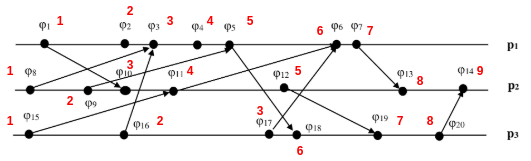
\includegraphics[width=\textwidth]{fig/4b.png}
\end{figure}


\begin{figure}[h]
    \centering
    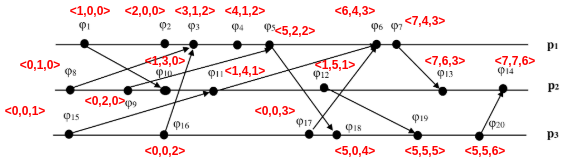
\includegraphics[width=\textwidth]{fig/4c.png}
\end{figure}

\section*{Exercise 4B(i)}
Let's have an example with two processes P1 and P2. P1 send a message
M1 to P2. The message M1 was delivered after a later-sent application
message. Because of this reordering, the recorded global state is
inconsistent

\section*{Exercise 4B(ii)}
By recording the messages in the process states, we can ignore
flushing channels. In this model, the original Chandy-Lamport
algorithm that assumes FIFO channels is:

\begin{lstlisting}[style=mycode]
Process 0: 
	Send "SS" to self

Process i: 
	when receive "SS" for first time (from pj):
		  record state
		  send "SS" to all neighbors
		  for each neighbor except pj wait for "SS"
\end{lstlisting}

To accommodate non-FIFO channels, we just have to ensure that the
delivery of the snapshot message does not get moved after the delivery
of subsequent messages. For this reason, we block sending application
messages until the snapshot is complete. We define a set BLOCK for
each process p. For each process q in BLOCK, p will block all sends to
q until q is no longer in BLOCK.

\begin{lstlisting}[style=mycode]
Process0: 
	send "SS" to self
Process i: 
	when receive "SS" for first time (from pj):
		  record state
		  BLOCK = all neighbors - { pj }
		  send "SS" to all neighbors
		  while (BLOCK != 0):
			  when receive "SS" (from pk)
			  BLOCK = BLOCK - { pk }
\end{lstlisting}


%------------------------------------------------
\end{document}

